\newcommand{\sps}{SCION PathStore\@\xspace}
\newcommand{\pse}{path-selection engine\@\xspace}
\newcommand{\PSE}{Path-selection Engine\@\xspace}
\newcommand{\qs}{queue snapshot\@\xspace}
\newcommand{\QS}{Queue Snapshot\@\xspace}
\newcommand{\sq}{SCION queue\@\xspace}
\newcommand{\SQ}{SCION Queue\@\xspace}
\newcommand{\BPS}{Best-path Set\@\xspace}
\newcommand{\bps}{best-path set\@\xspace}
\newcommand{\stride}{STRIDE\@\xspace}

\chapter{Path Store}
In this section, we describe {\em \bf SCION PathStore}, a data structure for storing SCION paths. We design \sps such that it would be used by both \BS and \CS.
The basic functionality of \sps is to store PCBs (which correspond to
SCION half-paths) in the local storage and to provide a set of paths
that best satisfy certain requirements.

{\bf \BS: } \BS stores all PCBs received from its upstream \ADs and at
each PCB propagation epoch, selects the best $k$ paths to propagate to
its customer \ADs. For this purpose, \BS evaluates the {\em path
  fidelity} (viz., Section~\ref{subsec:pcb_selection}) of each path
and maintain a list of $k$ paths that have the highest fidelity for
each customer \AD.

{\bf \PS: } \PS stores all up-paths received from the local \BS and on a client request, provides the best a set of paths that satisfy the client's request.

\begin{figure*}[th]
\centering
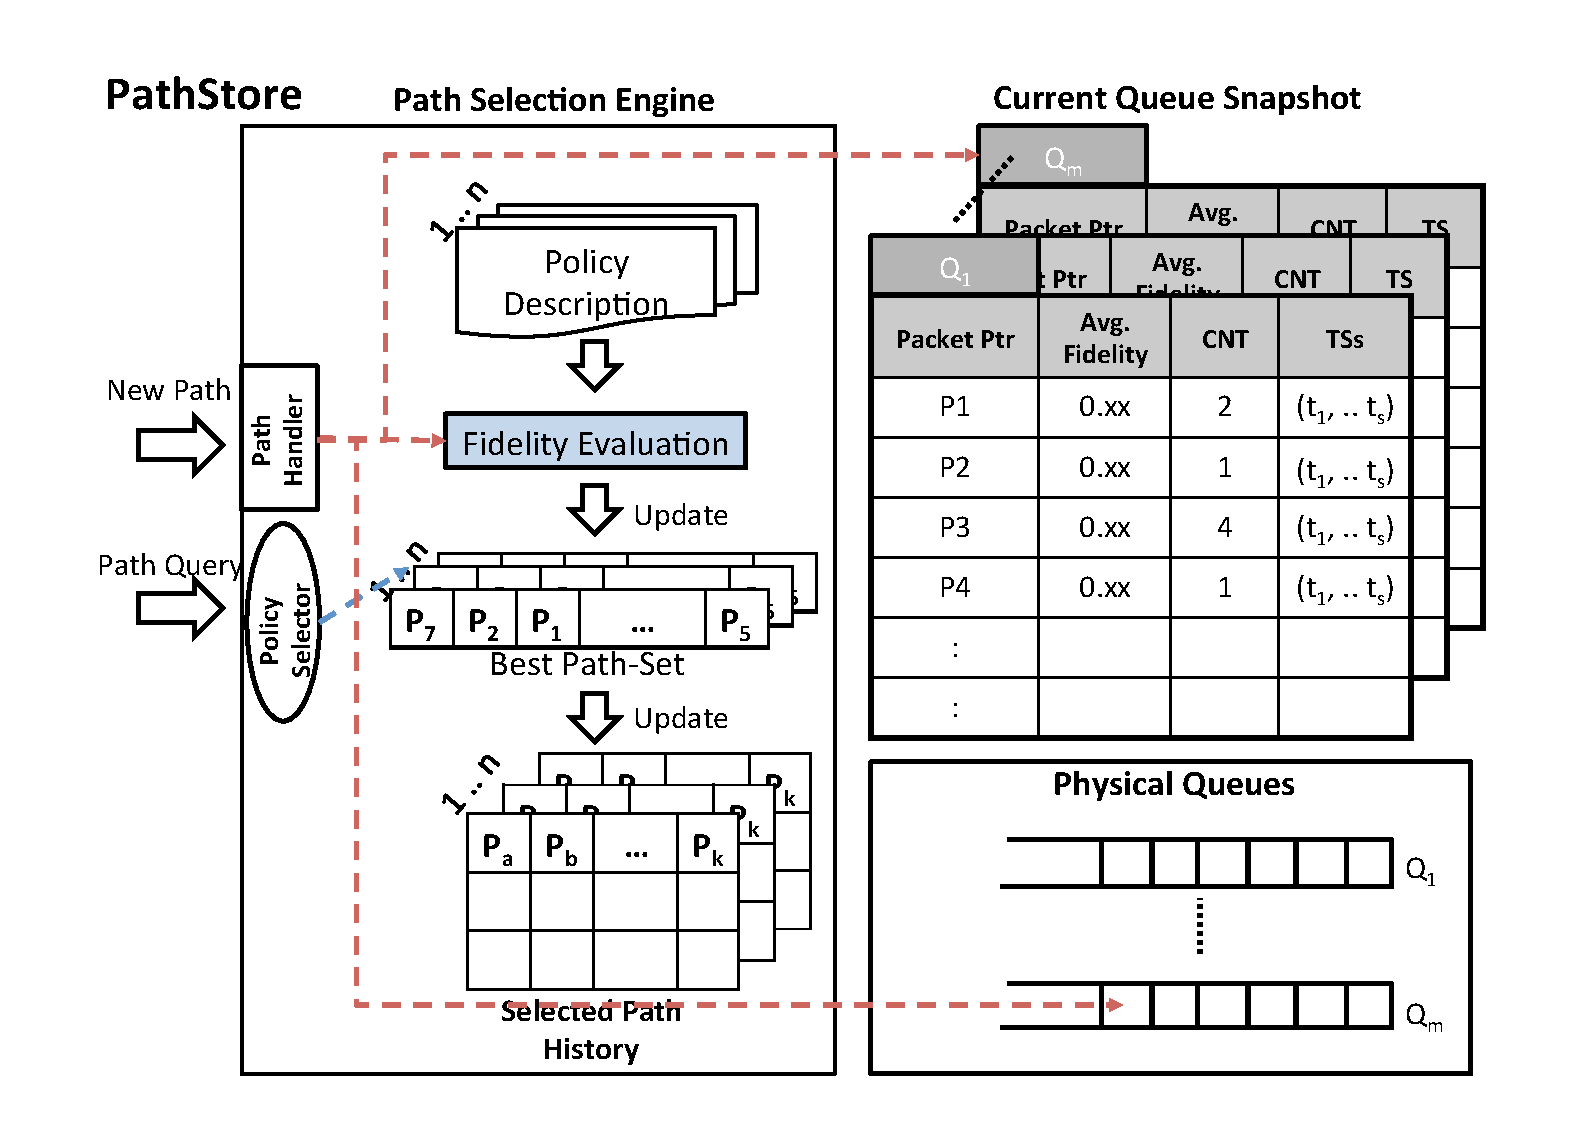
\includegraphics[width=.9\columnwidth]{./fig/path_store.eps}
\caption{Path Store.}~\label{fig:path_store}
\end{figure*}

\section{Overview}
\sps consists of three parts in large, which are \pse, \qs, and \sq. 

{\bf \PSE: } \PSE has a list of policies that describe the preference
of paths and a list best-path sets that correspond to individual
policies. For a new path, the \pse evaluates the path fidelity based
on each policy and adds this path to the corresponding best-path
set. The best-path set is sorted in the decreasing order of fidelity,
and the size of the best-set can be configured. For example, \BS sets
the size to $k$, where $k$ is the number of paths that would be
propagated to its customer \AD. \PSE stores the list of the selected
paths at a specific time in the path history table, by which the \pse
can evaluate path properties dependent on previous selection. Such
history-dependent path properties include path freshness and path
disjointness, as detailed in the next subsection. Storing exact copies
of selected paths in the path history table enables accurate
evaluation of history-dependent path properties, yet it introduces
high storage overhead. Hence, we need to consider some optimization
techniques to reduce storage overhead or to trade accuracy for
efficiency. For example, we may implement the path history table using
probabilistic data structures that give approximate results of
history-dependent properties.

{\bf \QS: } \QS keeps track of the digest of the paths that are currently in the queue (the queue can be either a packet buffer (in \BS) or a path database (in \PS)). This digest is used to select a path to drop when the current queue is full, and is constructed one for every queue. 

{\bf \SQ: } \sq manages the physical buffer where actual paths are stored. \sq supports fast enqueue/deque and automatic (intelligent) resize operations while maximally utilizing the physical memory. 

\section{Policy}~\label{subsec:policy}
A policy is defined by an administrator and read by the \pse during its initialization. A policy file defines the properties and their weights. The list of properties includes:

\begin{itemize}
\item{local desirability: } set by an \AD for the traffic engineering purpose
\item{path length: } path length in AS hops
\item{path freshness: } a value that indicates the arrival time of the path (integer value between 0 and MAX) \soobum{need to define this value}
\item{guaranteed bandwidth: } for capability request (\stride) 
\item{available bandwidth: } a value that reflects the current congestion status (\stride)
\item{total bandwidth: } the physical bandwidth of the path (\stride)
\item{delay/jitter: } each \AD annotates the maximum delay and jitter for a QoS service; this would be null for general services
\item{cost: } defined by a provider (different paths have different cost based on SLA)
\item{size: } the size of the best-path set; i.e., $m$ best paths.
\item{path disjointness: } the level of disjointness compared with
  previously selected paths
\end{itemize}

Once a policy defines properties ($R_i$) and their weights ($w_i$), Path Fidelity of a path $P_i$ is computed as:
\[
\textrm{Path Fidelity } F (P_i) = \sum w_i R_i
\]

Path fidelity captures a rich set of common path selection policies in
a form of a linear combination of the above properties. For example,
the Shortest-Path policy can be represented by setting the weight of
the path length to one and the rest to zeros.  However, path fidelity
itself fails short to represent blacklist- and whitelist-like policies
that exclude paths that meet or do not meet certain conditions. For
example, the administrator may want to avoid using paths that traverse
known malicious ISPs regardless of how good their path fidelity scores
are. Hence, a policy file also includes a filter (which can be defined
as a blacklist or whitelist) by which the \pse can remove unwanted
paths before computing path fidelity. Generally, a filter contains a
list of unwanted on-path ADs and the maximum and/or minimum values of
each path property.

As we describe earlier, the \pse maintains several policies and keeps
best paths for each of the policies. Hence, it does not scale if the
\pse has to maintain every possible policy. Instead, the \pse picks
and publishes a set of commonly used path selection policies (which
can be configured manually by the administrator). 

%path composition API
%avoid peer
%maximally disjoint path
%\item{trusted: } 

\section{Best-Path Set}~\label{subsec:bestpath}
If a new path is added to the queue, the \pse evaluates the path's fidelity for every policy and updates the corresponding best-path set. The best-path set keeps at most $m$ paths defined in the policy, hence it needs to remove one if the set is full. Whenever a path is added to or removed from the best-path set, the reference count (CNT in the figure) of the corresponding \qs is updated (increased/decreased). A path is removed from the queue only when its reference count becomes zero (no policy includes the path in its best-path set).
A path query is made with a predefined policy (we assume that the set of available policies are available to the requester; e.g., path propagation engine in BS, a client who request paths to PS), the \pse returns the \bps to the requester. The \pse creates a new \bps periodically, and after creating a new set, it stores the previous set in the path history table.
To avoid frequent best-path re-evaluation and corresponding overhead, the \pse computes the best-path sets either if a certain number of new paths are available or periodically.

\section{Current Queue Snapshot}~\label{subsec:queue-snapshot}
\QS contains the information of the paths that are currently in the queue. The information on a path $P_i$ includes:
\begin{itemize}
\item{Packet pointer (Packet Ptr): } the address of the packet (PCB) that corresponds to $P_i$
\item{Average Fidelity (Avg. Fidelity): } the average of fidelities of $P_i$ computed over all policies
\item{Reference Count (CNT): } the number of best-path set that includes a path $P_i$
\item{Timestamps (TSs): } the most recent $s$ queueing times of $P_i$
\end{itemize}
\QS is used to select a path to remove when the queue is full.

\section{SCION Queue}~\label{subsec:scion-queue}
\SQ is a base queue that is universally used by all SCION elements. The configuration parameters are as follows.

\begin{itemize}
\item number of queues and their lengths
\item priority/type of each queue; e.g., data, control (PCB), capability request
\item queue selection policy (e.g., Hash(Header) mod n, Path ID)
\item weight of each queue (e.g., for weighted FQ)
\end{itemize}

Other than the basic parameters listed above, SCION queue (may) support the following advanced funtionalities.

\begin{itemize}
\item intelligent queue? adjust/auto-set parameters based on traffic class; e.g., max delay, jitter, 
\item multi-layer (or hierarchical) queue; split/merge queues if necessary
\item stores average queue size (for queue management) and utilization (for bandwidth estimation)
\end{itemize}


